% Options for packages loaded elsewhere
\PassOptionsToPackage{unicode}{hyperref}
\PassOptionsToPackage{hyphens}{url}
%
\documentclass[
]{book}
\title{Open Science: An Introduction for Biology}
\author{}
\date{\vspace{-2.5em}2021-07-15}

\usepackage{amsmath,amssymb}
\usepackage{lmodern}
\usepackage{iftex}
\ifPDFTeX
  \usepackage[T1]{fontenc}
  \usepackage[utf8]{inputenc}
  \usepackage{textcomp} % provide euro and other symbols
\else % if luatex or xetex
  \usepackage{unicode-math}
  \defaultfontfeatures{Scale=MatchLowercase}
  \defaultfontfeatures[\rmfamily]{Ligatures=TeX,Scale=1}
\fi
% Use upquote if available, for straight quotes in verbatim environments
\IfFileExists{upquote.sty}{\usepackage{upquote}}{}
\IfFileExists{microtype.sty}{% use microtype if available
  \usepackage[]{microtype}
  \UseMicrotypeSet[protrusion]{basicmath} % disable protrusion for tt fonts
}{}
\makeatletter
\@ifundefined{KOMAClassName}{% if non-KOMA class
  \IfFileExists{parskip.sty}{%
    \usepackage{parskip}
  }{% else
    \setlength{\parindent}{0pt}
    \setlength{\parskip}{6pt plus 2pt minus 1pt}}
}{% if KOMA class
  \KOMAoptions{parskip=half}}
\makeatother
\usepackage{xcolor}
\IfFileExists{xurl.sty}{\usepackage{xurl}}{} % add URL line breaks if available
\IfFileExists{bookmark.sty}{\usepackage{bookmark}}{\usepackage{hyperref}}
\hypersetup{
  pdftitle={Open Science: An Introduction for Biology},
  hidelinks,
  pdfcreator={LaTeX via pandoc}}
\urlstyle{same} % disable monospaced font for URLs
\usepackage{longtable,booktabs,array}
\usepackage{calc} % for calculating minipage widths
% Correct order of tables after \paragraph or \subparagraph
\usepackage{etoolbox}
\makeatletter
\patchcmd\longtable{\par}{\if@noskipsec\mbox{}\fi\par}{}{}
\makeatother
% Allow footnotes in longtable head/foot
\IfFileExists{footnotehyper.sty}{\usepackage{footnotehyper}}{\usepackage{footnote}}
\makesavenoteenv{longtable}
\usepackage{graphicx}
\makeatletter
\def\maxwidth{\ifdim\Gin@nat@width>\linewidth\linewidth\else\Gin@nat@width\fi}
\def\maxheight{\ifdim\Gin@nat@height>\textheight\textheight\else\Gin@nat@height\fi}
\makeatother
% Scale images if necessary, so that they will not overflow the page
% margins by default, and it is still possible to overwrite the defaults
% using explicit options in \includegraphics[width, height, ...]{}
\setkeys{Gin}{width=\maxwidth,height=\maxheight,keepaspectratio}
% Set default figure placement to htbp
\makeatletter
\def\fps@figure{htbp}
\makeatother
\setlength{\emergencystretch}{3em} % prevent overfull lines
\providecommand{\tightlist}{%
  \setlength{\itemsep}{0pt}\setlength{\parskip}{0pt}}
\setcounter{secnumdepth}{5}
\ifLuaTeX
  \usepackage{selnolig}  % disable illegal ligatures
\fi
\usepackage[]{natbib}
\bibliographystyle{apalike}

\begin{document}
\maketitle

{
\setcounter{tocdepth}{1}
\tableofcontents
}
\hypertarget{part-os-101}{%
\part*{OS 101}\label{part-os-101}}
\addcontentsline{toc}{part}{OS 101}

\hypertarget{welcome}{%
\chapter*{Welcome}\label{welcome}}
\addcontentsline{toc}{chapter}{Welcome}

This text was built to accompany the first year of the Biology undergraduate degree program at UBC Okanagan. It's aim is to introduce learners to core considerations in the pursuit of open scientific practices. It's divided into three sections, the first exploring principles and concepts associated with Open Science, the second and third looking at these principles and concepts in practice.

Part 1, \emph{Principles of Open Science} will be covered in BIOL 116. Parts 2 and 3, \emph{Open Science in Action: Benefits} and \emph{Open Science in Action: Challenges}, will be covered in BIOL 125.

\hypertarget{copyright}{%
\section*{Copyright}\label{copyright}}
\addcontentsline{toc}{section}{Copyright}

This work is licenced under the Creative Commons \href{https://creativecommons.org/licenses/by-nc-sa/4.0/}{Attribution-NonCommercial-ShareAlike 4.0 International (CC BY-NC-SA 4.0)}

Please use the following for citing this document

Hanna, S., Pither, J., Vis-Dunbar, M. (2021). \emph{Open Science. An introduction for Biology}. \href{}{https://SOMETHING HERE}

All source files are available \href{}{here}.

\hypertarget{conventions}{%
\section*{Conventions}\label{conventions}}
\addcontentsline{toc}{section}{Conventions}

In text:

\begin{itemize}
\tightlist
\item
  \href{}{hyperlinked terms} take the user to a glossary in the UBCO Biology Department's \href{}{Procedures \& Guidelines} ebook.
\end{itemize}

Glyhps:

\begin{longtable}[]{@{}ll@{}}
\toprule
\endhead
& Lab exercises for discussion \\
& Examples of principles in practice \\
& Highlight of UBC researcher engaged or participating in Open Science \\
\bottomrule
\end{longtable}

\hypertarget{principles-of-open-science}{%
\chapter{Principles of Open Science}\label{principles-of-open-science}}

\hypertarget{the-burden-of-proof}{%
\section{The Burden of Proof}\label{the-burden-of-proof}}

Science is a beautiful thing. It is a landscape of exploration and one that at its root is tasked with finding evidence, and establishing cause and effect. At a fundamental level, this implies that science should be able to answer questions like these.

\begin{quote}
If I exercise daily, how is this likely to affect my cardiovascular (heart) health?

If we build a road here, how will the local population of bighorn sheep be affected?
\end{quote}

As you'll discover throughout your degree, scientists tackle such questions through a combination of exploratory research and confirmatory research. At the exploratory stage, ideas are generated and associations are discovered. Exploratory research gives rise to hypotheses that can then be tested through confirmatory research, which requires well-designed experiments. For instance, based on observation, we have long hypothesized that there are positive associations between exercise and physical health. But establishing that daily exercise causes healthy outcomes is a different challenge.

Many research teams have designed studies to address various aspects of these observed benefits of physical activity. One such team, an interdisciplinary research team at UBC, tackled this question in relation to falls in an aging population \citep{liu-ambrose_effect_2019}. The researchers designed an experiment to to test whether strength training after experiencing a fall in an aging population would reduce injuries from a subsequent fall.

\hypertarget{exercise-and-positive-health-outcomes}{%
\paragraph*{Exercise and Positive Health Outcomes}\label{exercise-and-positive-health-outcomes}}
\addcontentsline{toc}{paragraph}{Exercise and Positive Health Outcomes}

After reading the following abstract from Liu-Ambrose et al's paper \emph{Effect of a Home-Based Exercise Program on Subsequent Falls Among Community-Dwelling High-Risk Older Adults After a Fall} \citep{liu-ambrose_effect_2019}, try and answer the following questions.

\begin{itemize}
\tightlist
\item
  Was this study confirmatory or exploratory? How do we know this?
\item
  Who participated in the study?
\item
  What was the intervention?
\item
  What were the main conclusions?
\end{itemize}

\hypertarget{abstract}{%
\paragraph*{Abstract}\label{abstract}}
\addcontentsline{toc}{paragraph}{Abstract}

\textbf{Importance} Whether exercise reduces subsequent falls in high-risk older adults who have already experienced a fall is unknown.

\textbf{Objective} To assess the effect of a home-based exercise program as a fall prevention strategy in older adults who were referred to a fall prevention clinic after an index fall.

\textbf{Design, Setting, and Participants} A 12-month, single-blind, randomized clinical trial conducted from April 22, 2009, to June 5, 2018, among adults aged at least 70 years who had a fall within the past 12 months and were recruited from a fall prevention clinic.

\textbf{Interventions} Participants were randomized to receive usual care plus a home-based strength and balance retraining exercise program delivered by a physical therapist (intervention group; n = 173) or usual care, consisting of fall prevention care provided by a geriatrician (usual care group; n = 172). Both were provided for 12 months.

\textbf{Main Outcomes and Measures} The primary outcome was self-reported number of falls over 12 months. Adverse event data were collected in the exercise group only and consisted of falls, injuries, or muscle soreness related to the exercise intervention.

\textbf{Results} Among 345 randomized patients (mean age, 81.6 {[}SD, 6.1{]} years; 67\% women), 296 (86\%) completed the trial. During a mean follow-up of 338 (SD, 81) days, a total of 236 falls occurred among 172 participants in the exercise group vs 366 falls among 172 participants in the usual care group. Estimated incidence rates of falls per person-year were 1.4 (95\% CI, 0.1-2.0) vs 2.1 (95\% CI, 0.1-3.2), respectively. The absolute difference in fall incidence was 0.74 (95\% CI, 0.04-1.78; P = .006) falls per person-year and the incident rate ratio was 0.64 (95\% CI, 0.46-0.90; P = .009). No adverse events related to the intervention were reported.

\textbf{Conclusions and Relevance} Among older adults receiving care at a fall prevention clinic after a fall, a home-based strength and balance retraining exercise program significantly reduced the rate of subsequent falls compared with usual care provided by a geriatrician. These findings support the use of this home-based exercise program for secondary fall prevention but require replication in other clinical settings.

\textbf{Trial Registration} ClinicalTrials.gov Identifiers: NCT01029171; NCT00323596

\hypertarget{causal-links}{%
\subsection*{Causal Links}\label{causal-links}}
\addcontentsline{toc}{subsection}{Causal Links}

Suggesting a causal link brings with it the need to show your proof. This burden of scientific proof requires both creativity and rigour; studies must be well designed and well executed. It also requires that studies be independently replicated to show that, if repeated, they will result in the same conclusions, reinforcing the validity of the original findings. On the other hand, a replication study may come to a different conclusion, potentially invalidating the conclusions of the original study.

Say, for example, that you're provided with the choice between two medications to treat a medical condition you'd prefer wasn't mentioned in a publicly available education resource. Neither has a record of adverse side effects, but one drug, we'll be creative and call it "drug A" has findings obtained from only a single research lab, while "drug B" underwent five independently replicated studies in five different labs with five independent researchers. Which medication might you choose?

\hypertarget{science-social-trust}{%
\subsection*{Science \& Social Trust}\label{science-social-trust}}
\addcontentsline{toc}{subsection}{Science \& Social Trust}

Science does not exist independent of the rest of society. The outputs of science --- the discoveries made through research --- answer questions we have in all facets of life.

\begin{quote}
What is a healthy lunch option?

Is lead-based paint safe?

What's the safest way to perform heart surgery?

What should government policy be on climate change?
\end{quote}

If science is going to be used by the public, other scientists, and policy makers to address these questions, they need to be able both to gain access to and to trust these findings.

\hypertarget{trust-access}{%
\subsubsection*{Trust \& Access}\label{trust-access}}
\addcontentsline{toc}{subsubsection}{Trust \& Access}

Scientists can build public trust in science through the use of

\begin{itemize}
\tightlist
\item
  rigour in the scientific method and
\item
  replication (thorough repetition) of studies to build and solidify the evidence for a conclusion.
\end{itemize}

We can assure access to science by removing barriers to access, such as fees for articles, and by tailoring communication of the outputs for specific audiences.

\hypertarget{stakeholders-in-science}{%
\subsubsection*{Stakeholders in Science}\label{stakeholders-in-science}}
\addcontentsline{toc}{subsubsection}{Stakeholders in Science}

Designing accessible outputs for a particular audience means considering the prior knowledge, education, and needs of different stakeholders in science.

Who exactly is a stakeholder? Anyone who can influence or be affected by a matter. Examples of these could include government policy makers and funders, business and industry, politicians, environmentalists, patients, and the general public.

\hypertarget{a-crisis}{%
\section{A Crisis}\label{a-crisis}}

Much of the scientific community was shocked in 2005 when researcher, John Ioannidis \citep{ioannidis_why_2005}, wrote a paper claiming that most published research findings are false.

Ioannidis was criticizing the rigour of the scientific process used by researchers in medicine. His statement sparked a movement that started questioning whether or not published studies could be replicated: that is, could they withstand a test of their burden of proof?

Since Ioannidis published his paper, this movement has grown into a crusade seeking to transform the culture and practices of scientific research. As a society and as a species we face many challenges that require us to work together across geographical, social, political, and disciplinary boundaries. Solid science and public confidence in that science figure prominently in efforts to address such issues as health and wellness, climate change, and the need to make resource use sustainable. What's needed is a change in culture and practices to improve knowledge sharing, quality, accessibility, and trust in science.

\hypertarget{why-most-published-research-findings-are-false}{%
\paragraph*{Why Most Published Research Findings are False}\label{why-most-published-research-findings-are-false}}
\addcontentsline{toc}{paragraph}{Why Most Published Research Findings are False}

After reading the following abstract from John Ioannidis's article \citep{ioannidis_why_2005}, reflect on the following questions.

\begin{itemize}
\tightlist
\item
  What factors did Ioannidis identify for the lack of reliability in research studies?
\item
  How might these problems be addressed?
\end{itemize}

\hypertarget{abstract-1}{%
\paragraph*{Abstract}\label{abstract-1}}
\addcontentsline{toc}{paragraph}{Abstract}

There is increasing concern that most current published research findings are false. The probability that a research claim is true may depend on study power and bias, the number of other studies on the same question, and, importantly, the ratio of true to no relationships among the relationships probed in each scientific field.

In this framework, a research finding is less likely to be true when the studies conducted in a field are smaller; when effect sizes are smaller; when there is a greater number and lesser preselection of tested relationships; where there is greater flexibility in designs, definitions, outcomes, and analytical modes; when there is greater financial and other interest and prejudice; and when more teams are involved in a scientific field in chase of statistical significance. Simulations show that for most study designs and settings, it is more likely for a research claim to be false than true. Moreover, for many current scientific fields, claimed research findings may often be simply accurate measures of the prevailing bias. In this essay, I discuss the implications of these problems for the conduct and interpretation of research.

\hypertarget{what-exactly-is-open-science}{%
\section{What Exactly is Open Science?}\label{what-exactly-is-open-science}}

In the previous sections we discussed the burden of proof and the erosion of social and stakeholder trust in the sciences.

This next section will explore a related issue: the ability to build up evidence for a scientific claim by repeating the original study to make sure that the finding, be it correlative or causal, is a true finding and not just a fluke.

\hypertarget{a-replication-crisis}{%
\subsection*{A Replication Crisis}\label{a-replication-crisis}}
\addcontentsline{toc}{subsection}{A Replication Crisis}

Open Science proposes many solutions to problems with how research is done. It aims to ensure that research can be confirmed through replication, and that both new discoveries and replications of previous research are respected and rewarded.

\hypertarget{replication}{%
\subsubsection*{Replication}\label{replication}}
\addcontentsline{toc}{subsubsection}{Replication}

Although scientific progress rests on the repetition and reproduction of results, efforts at this are hindered by two main factors.

\begin{itemize}
\tightlist
\item
  First, there is a desire for the new and shiny: novel studies are more interesting.
\item
  Secondly, many studies cannot be competently analyzed or replicated. This is because critical information about them --- design, data, methods, lab notes, analyses and code --- may not be made available, or may be poorly communicated.
\end{itemize}

\hypertarget{flashy-science-or-good-science}{%
\subsection*{Flashy Science or Good Science}\label{flashy-science-or-good-science}}
\addcontentsline{toc}{subsection}{Flashy Science or Good Science}

New, positive, and original findings are exciting. Independently repeating a study and getting the same results, not so much. The consequence for science? New, positive, and flashy findings get published and a lot of attention. Re-testing, or replicating these studies, and non-positive findings often attract much less attention.

The result? Novel research gets funded and published. Sometimes, it appears, the excitement factor overrides the quality (or lack of quality) of the science.

\hypertarget{incentives}{%
\subsection*{Incentives}\label{incentives}}
\addcontentsline{toc}{subsection}{Incentives}

Replication studies are hard to fund, and many journals are not interested in publishing them. And universities and scientific institutes offer career rewards to those who publish novel findings in prestigious journals.

Academia and industry alike reward the publication of positive and so-called "significant" results. Scientists may unwittingly "bend the rules" of science trying to get results worthy of publication. "Bending the rules" in this context is also known as engaging in Questionable Research Practices (QRPs).

\hypertarget{questionable-research-practices}{%
\subsubsection*{Questionable Research Practices}\label{questionable-research-practices}}
\addcontentsline{toc}{subsubsection}{Questionable Research Practices}

It's important to note that QRPs don't normally result from deliberate efforts on the part of researchers to do bad science. QRPs arise from a complex system of interactions within and around the research process and from the need for researchers to get published. After all, publications are the bread and butter of a researcher. And unfortunately, this can mean that sometimes style trumps substance, as Daniel Engber notes in his \emph{Slate} article "Cancer Research Is Broken" \citep{engber_cancer_2016}.

\hypertarget{enter-open-science}{%
\subsection*{Enter Open Science}\label{enter-open-science}}
\addcontentsline{toc}{subsection}{Enter Open Science}

Open Science is a movement that tries to combat the replication crisis, QRPs, and style trumping substance in two ways:

\begin{itemize}
\tightlist
\item
  by providing different incentives and rewards for research. That is, changing what we measure as a success in research, shifting from a culture that emphasizes novel findings to one that also rewards the many other aspects of practicing good science;
\item
  by making all parts of the scientific research process transparent and accessible, allowing for a critical review of how a study was conducted, and ultimately enabling that study to be independently replicated.
\end{itemize}

\hypertarget{open-science-ideals}{%
\subsubsection*{Open Science Ideals}\label{open-science-ideals}}
\addcontentsline{toc}{subsubsection}{Open Science Ideals}

What sort of changes, then, would we expect Open Science to bring? Imagine a world where

\begin{itemize}
\tightlist
\item
  publications and data are freely available \footnote{There are some necessary and reasonable restrictions on data availability, such as privacy concerns, cultural and intellectual property rights, or even protection of the location of endangered species, to name a few.};
\item
  conclusions and public policy are based on solid information and analysis that are clearly evident to all;
\item
  studies can be tested and repeated;
\item
  researchers without extensive funding or resources can still participate and collaborate in science;
\item
  good science --- rather than flashy science --- brings rewards to those who practice it; and
\item
  the public trusts science and has opportunities to participate in research.
\end{itemize}

\hypertarget{core-values}{%
\section{Core Values}\label{core-values}}

In the previous section we talked about the relationship between science and society, and tried to imagine an ideal research landscape transformed by Open Science. In this section we'll dive a little deeper and get to the core beliefs that underlie OS principles and practices.

The fundamental values we'll look at include

\begin{itemize}
\tightlist
\item
  scientific quality and integrity;
\item
  equity;
\item
  communication; and
\item
  diversity and inclusion.
\end{itemize}

\hypertarget{core-values-scientific-integrity}{%
\section{Core Values: Scientific Integrity}\label{core-values-scientific-integrity}}

Though we haven't mentioned the phrase "scientific integrity", we have looked at the critical role it plays in replicability and Open Science. Integrity involves sticking to best practices for research that promote reproducibility through transparency and open access. At its root, this principle springs from a sense of responsibility for public welfare and from the honest pursuit of scientific truth.

In a literal sense, transparency is the property of an object that makes it so clear that you can see through it. But what about when we talk about transparency in government policy, or scientific research? In this context, transparency implies a high degree of disclosure --- revealing clearly the exact reasoning and process used in coming to a decision or taking an action. As well, transparency means taking care to disclose important information in a respectful and responsible fashion.

\hypertarget{best-practices}{%
\subsection*{Best Practices}\label{best-practices}}
\addcontentsline{toc}{subsection}{Best Practices}

Scientific integrity implies several practices:

\begin{itemize}
\tightlist
\item
  basing research conclusions and public policy on solid information and analyses that are clearly evident to everyone;
\item
  evaluating scientific work using fair, rigorous criteria and procedures known to all involved;
\item
  publishing good science, period (not just flashy science);
\item
  fully disclosing study methods and outcomes regardless of the findings being "significant";
\item
  following best practices for creating hypotheses, collecting data, and analyzing results;
\item
  demonstrating sensitivity to stakeholders' ownership of knowledge and data; and
\item
  providing equitable access to all outputs of the research cycle.
\end{itemize}

As we saw in the last section, these form key elements of our ideal research ecosystem, where the public trusts science and studies can be tested and repeated.

\hypertarget{transparency-grading}{%
\paragraph*{Transparency \& Grading}\label{transparency-grading}}
\addcontentsline{toc}{paragraph}{Transparency \& Grading}

One case where students want and need transparency is in grading. Most of you probably appreciate knowing how marks were given to questions on a midterm exam and what criteria the marker used to score each question. This provides you with both a \emph{reason} for the assigned grade and a means of \emph{comparing} your grade with those of your classmates.

Ultimately, this specific information can help you to address gaps in your knowledge and perform better on future assessments (such as the final exam). In the same way, transparency in research allows scientists to improve future studies and add to accumulated knowledge.

\hypertarget{core-values-equity-communication}{%
\section{Core Values: Equity \& Communication}\label{core-values-equity-communication}}

What is equity? Does equity equal equality?

Equity and equality are similar, but there is a key distinction: under equality everyone is treated in an identical manner, whereas under equity everyone is treated fairly according to their abilities and needs.

The following image nicely illustrates the concept of equity:

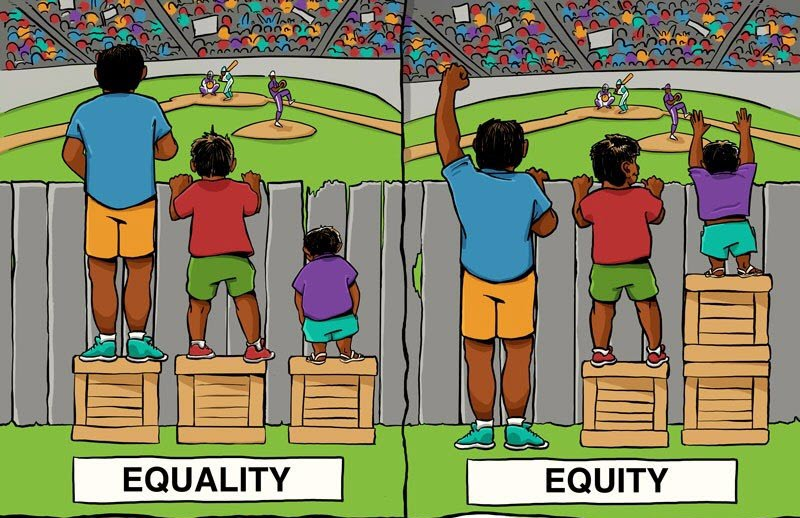
\includegraphics{images/equity_cropped.jpg}

Image attribution: \href{https://www.flickr.com/photos/leighblackall/30727349115/}{Universalincome} {[}cropped{]} by \href{https://www.flickr.com/photos/leighblackall/}{Leigh Blackall} under \href{https://creativecommons.org/licenses/by/2.0}{Attribution 2.0 Generic (CC BY 2.0)}.

\hypertarget{communication}{%
\subsection*{Communication}\label{communication}}
\addcontentsline{toc}{subsection}{Communication}

We do research to learn; we share our findings to build a culture of learning and to enhance the future of our disciplines. We also share to build community with researchers and other stakeholders.

But because there can be a range of stakeholders with different needs, values, and backgrounds, it is important to communicate science in ways that consider these specific attributes. Processes and findings need to be \emph{contextualized} (put into a context meaningful to the particular stakeholder) and \emph{made accessible}, both in message (the content of the communication) and medium (the way the message is conveyed). The more avenues we use to share and engage and the fewer barriers to access we put up, the more equitably our discoveries can be shared.

Equity in science communication can be explored in many ways; none addresses all issues of equitable access, but each helps to enhance scientific literacies in our society.

\begin{itemize}
\tightlist
\item
  Open access publications help to make research available to those who cannot afford costly journal subscriptions.
\item
  Citizen science engages members of the public in the research process, contributing their voices to projects.
\item
  Novel ways of sharing a message, like podcasts or Twitter, can reach communities with unique access needs or preferences.
\end{itemize}

\hypertarget{audiences}{%
\subsection*{Audiences}\label{audiences}}
\addcontentsline{toc}{subsection}{Audiences}

The language and techniques your Biology professor uses to communicate scientific information will vary according to her audience. Depending on whom she's interacting with, your Biology professor will use different language and techniques to convey scientific information. For example, in the course of her work, she may be

\begin{itemize}
\tightlist
\item
  engaging you and your classmates in learning in the classroom;
\item
  talking to a member of the public;
\item
  working on research with a departmental colleague; or
\item
  advising a government employee involved in writing policy.
\end{itemize}

In each case, she adjusts her communication to match her audience's needs, educational background, and experience. Her message isn\textbackslash't fundamentally changed or simplified, but it does need to be delivered in a way that is understanding and respectful of her audience.

\hypertarget{effects-of-ddt-on-birds-three-approaches}{%
\paragraph*{Effects of DDT on Birds: Three Approaches}\label{effects-of-ddt-on-birds-three-approaches}}
\addcontentsline{toc}{paragraph}{Effects of DDT on Birds: Three Approaches}

Consider each of the following three explanations of how DDT affects birds in terms of its intended audience.

\textbf{Aimed at Researchers in the Discipline}

Dichlorodiphenyltrichloroethane (DDT) is a persistent organochlorine compound found worldwide that causes significant anatomical, physiological and behavioural abnormalities in humans and wildlife \citep{iwaniuk_effects_2006}.

\textbf{Aimed at Post-Secondary Science Students}

DDT and its metabolites cause eggs to have thin shells and reduce levels of a hormone necessary for female birds to lay eggs. Population declines and local disappearance of peregrine falcons, bald and golden eagles, ospreys, kestrels, and other predatory birds were recorded \citep{cox_pesticides_1991}.

\textbf{Aimed at the General Public}

High concentrations of DDT in birds cause weakness in the shells of their eggs, which leads to a reduction in their population. DDT is now banned because of this \citep{bbc_bitesize_food_nodate}.

\hypertarget{core-values-diversity-inclusion}{%
\section{Core Values: Diversity \& Inclusion}\label{core-values-diversity-inclusion}}

You've almost certainly heard these terms, but may wonder if there's a difference between them.

In the context of Open Science diversity is the practice or quality of engaging in research with individuals who vary in terms of social class, ethnic background, sexual orientation, gender, ability, etc.

Inclusion takes this diverse engagement further: it looks at the individual in relation to the community, organization, or society, and ensures that they not only participate in, but guide the research process, especially as the research impacts these diverse communities as stakeholders in the research process and the implementation of findings from research.

Looking back at our discussion in the previous section, diversity and inclusion seem to be natural partners of equity.

\hypertarget{diversity-in-research-culture}{%
\subsection*{Diversity in Research Culture}\label{diversity-in-research-culture}}
\addcontentsline{toc}{subsection}{Diversity in Research Culture}

Diverse criticism of scientific ideas makes research more robust, and challenges biases and assumptions that might otherwise pass unchecked.

Divergent perspectives, skill sets, and ideas introduce the "outside-of-the-box" thinking that drives research forward. Involving a diversity of views and people enriches research.

Diversity and inclusion show up in many types of research activities that involve participation and collaboration. Participation and collaboration can take many forms.

\begin{itemize}
\tightlist
\item
  Citizen science engages the public in data collection and processing.
\item
  Partnership research turns the relationship between researcher and subject into a partnership, where both contribute to the research question, methods, and outcomes.
\item
  International collaborations increase cultural diversity and can address problems that cross borders, like disease epidemics or pollution.
\item
  Interdisciplinary research, such as collaborations between medical researchers on the one hand and veterinarians and animal specialists on the other, can help investigate complex questions like how the COVID-19 coronavirus evolves in intermediate hosts before being transferred to humans.
\end{itemize}

\hypertarget{partnership-research-integrated-knowledge-translation-ikt}{%
\paragraph*{Partnership Research: Integrated Knowledge Translation (IKT)}\label{partnership-research-integrated-knowledge-translation-ikt}}
\addcontentsline{toc}{paragraph}{Partnership Research: Integrated Knowledge Translation (IKT)}

Historically, there has been an imbalanced power relationship between people with differing physical abilities or medical conditions and the experts responsible for their care, medical treatment or research of their conditions.

In recent years, however, patient rights movements have focused on returning power to people undergoing medical care. And researchers and practitioners are adapting their practices, recognizing that people living with a medical condition hold unique knowledge about how it affects them, and this lived experience can be used to improve both research and outcomes.

An interdisciplinary panel of researchers from both UBC campuses, led by Dr.~Kathleen Martin-Ginis, has engaged with people living with spinal cord injury (SCI) to set up guidelines for collaboration that give those with SCI a voice in the research process, from the choice of avenues to investigate to decisions on the implementation of research results. This model of collaborative research, which is known as Integrated Knowledge Translation, has been shown to \citep{gainforth_integrated_2021}:

\begin{itemize}
\tightlist
\item
  improve the quality of science;
\item
  increase the probability that findings will be used in real life in policy or practice;
\item
  facilitate learning among all parties involved; and
\item
  make research more relevant to patient needs.
\end{itemize}

You can check out one output from this research, the \href{http://ok-ikt-2019.sites.olt.ubc.ca/files/2021/02/IKT_Guiding_Principles_Feb_2021_1.pdf}{Integrated Knowledge Translation (IKT) Guiding Principles for Conducting Spinal Cord Injury (SCI) Research in Partnership.}

\hypertarget{an-equitable-and-inclusive-open-science}{%
\section{An Equitable and Inclusive Open Science}\label{an-equitable-and-inclusive-open-science}}

In the past few years, the core values of equity, diversity, and inclusion have come to play an increasingly important role in the Open Science movement. It has also begun to recognize and account for the legacy of colonization: the historical, ingrained differences in power that exist between the Global North and Global South, among countries, and within countries between dominant groups and those that have been marginalized.

Sometimes, solutions involve using multiple ways of knowing to make and carry out science policy.

\hypertarget{government-policy-diverse-teams-informing-species-risk-assessment}{%
\paragraph*{Government Policy:~Diverse Teams Informing Species Risk Assessment}\label{government-policy-diverse-teams-informing-species-risk-assessment}}
\addcontentsline{toc}{paragraph}{Government Policy:~Diverse Teams Informing Species Risk Assessment}

Dr.~Jeannette Armstrong was born and raised in the South Okanagan, on the Penticton Indian reserve. Dr.~Armstrong is well known as an author, poet, educator, and Indigenous rights activist.

At UBC Okanagan, she holds a Canada Research Chair in Okanagan Indigenous Knowledge and Philosophy. She is also one of several people on a subcommittee of The Committee on the Status of Endangered Wildlife in Canada (COSEWIC), which advises the Minister of Environment and Climate Change Canada on designation of species at risk \citep{li_jeannettes_nodate} \citep{committee_on_the_status_of_endangered_wildlife_in_canada_atk_nodate}.

The \href{https://cosewic.ca/index.php/en-ca/about-us/cosewic-subcommittees}{COSEWIC website} states:

\begin{quote}
Incorporating Aboriginal Traditional Knowledge into COSEWIC's assessment of species at risk improves the process, and therefore the quality of designations made by COSEWIC, by bringing information and perspectives on wildlife species that are not available in published scientific literature.
\end{quote}

\hypertarget{countering-systemic-bias}{%
\subsection*{Countering Systemic Bias}\label{countering-systemic-bias}}
\addcontentsline{toc}{subsection}{Countering Systemic Bias}

However, more work is needed to really shift the systemic imbalance that has resulted from the legacies of our society holding the white, heterosexual, male, middle-class or higher, able-bodied adult up as the "norm" --- the norm around which our society constructs its practices and institutions, including its universities, employment law, and research design, to name a few. When this favouritism is enshrined in legislation, administrative processes, career advancements, our education systems, etc., we call it systemic bias.

If we differ in terms of any of the characteristics listed above --- whether in our ethnicity, gender, sexual orientation, social class, or ability --- we lack that the level of privilege their possession confers. Equitable practices try to shift this imbalance.

Systemic bias, and the norms these biases engender, infiltrate many aspects of how research is undertaken. Sometimes this manifests in the conduct of science itself, where as recently as the end of the Second World War, some scientists helped to promote "scientific racism", encoding these norms through taxonomies and classification systems that grouped humankind into different races. Another discipline that we would now call "pseudoscience", phrenology, attempted to correlate intelligence and personality to observable features of the human skull.

This discriminatory system, as we've discussed, can even prevent people from engaging in the practice of scientific research from the outset.

\hypertarget{indigenous-representation-in-science}{%
\paragraph*{Indigenous Representation in Science}\label{indigenous-representation-in-science}}
\addcontentsline{toc}{paragraph}{Indigenous Representation in Science}

\href{https://www12.statcan.gc.ca/census-recensement/2016/as-sa/fogs-spg/Facts-cma-eng.cfm?LANG=Eng\&GK=CMA\&GC=915\&TOPIC=9}{In 2016, 6\% of Kelowna's population identified as Aboriginal} (a term including a number of more specific Indigenous identities, such as Metis, Inuk, and First Nations). If there were no bias in the school and post-secondary educational systems, and assuming that Indigenous people are just as capable as non-Indigenous people at doing science, we would expect to see a comparable percentage of Indigenous people studying and teaching science in colleges and universities. But we don't.

\hypertarget{discussion-question}{%
\paragraph*{Discussion Question}\label{discussion-question}}
\addcontentsline{toc}{paragraph}{Discussion Question}

Consider the following questions.

\begin{itemize}
\tightlist
\item
  What implications might this have for how research is conducted at UBC?
\item
  How can we change this?
\end{itemize}

\hypertarget{wrap-up}{%
\section{Wrap up}\label{wrap-up}}

This has been a very short introduction to the world of Open Science; the crisis that launched a movement to address underlying issues in reproducibility, transparency, access, and equity and diversity in scientific research.

In subsequent chapters and terms, we'll explore some of the challenges researchers face in implementing practices related to Open Science as well as some of the successes that have emerged from within UBC as our faculty and students embrace methods for well done research rooted in transparent, reproducible methods that integrate alternative ways of viewing our environments, and evaluate research goals and outcomes base on diverse perspectives that result from different experiences.

\hypertarget{references}{%
\chapter{References}\label{references}}

  \bibliography{OS-Basics.bib}

\end{document}
